%%%%%%%%%%%%%%%%%%%%%%%%%%%%%%%%%%%%%%%%%
% Short Sectioned Assignment
% LaTeX Template
% Version 1.0 (5/5/12)
%
% This template has been downloaded from:
% http://www.LaTeXTemplates.com
%
% Original author:
% Frits Wenneker (http://www.howtotex.com)
%
% License:
% CC BY-NC-SA 3.0 (http://creativecommons.org/licenses/by-nc-sa/3.0/)
%
%%%%%%%%%%%%%%%%%%%%%%%%%%%%%%%%%%%%%%%%%

%----------------------------------------------------------------------------------------
%	PACKAGES AND OTHER DOCUMENT CONFIGURATIONS
%----------------------------------------------------------------------------------------

\documentclass[paper=a4, fontsize=11pt]{scrartcl} % A4 paper and 11pt font size

\usepackage[T1]{fontenc} % Use 8-bit encoding that has 256 glyphs
\usepackage{fourier} % Use the Adobe Utopia font for the document - comment this line to return to the LaTeX default
\usepackage[english]{babel} % English language/hyphenation
\usepackage{amsmath,amsfonts,amsthm} % Math packages
\usepackage{slashed}

\usepackage{graphicx}
\usepackage{multicol}
\usepackage{enumitem}
\usepackage{caption}
\usepackage{esint}

\usepackage{listings}
\usepackage{color}

\definecolor{dkgreen}{rgb}{0,0.6,0}
\definecolor{gray}{rgb}{0.5,0.5,0.5}
\definecolor{mauve}{rgb}{0.58,0,0.82}

\lstset{frame=tb,
  language=C,
  aboveskip=3mm,
  belowskip=3mm,
  showstringspaces=false,
  columns=flexible,
  basicstyle={\small\ttfamily},
  numbers=none,
  numberstyle=\tiny\color{gray},
  keywordstyle=\color{blue},
  commentstyle=\color{dkgreen},
  stringstyle=\color{mauve},
  breaklines=true,
  breakatwhitespace=true
  tabsize=3
}

\usepackage{lipsum} % Used for inserting dummy 'Lorem ipsum' text into the template

\usepackage{sectsty} % Allows customizing section commands
\allsectionsfont{\centering \normalfont\scshape} % Make all sections centered, the default font and small caps

\usepackage{abstract}
\renewcommand{\abstractnamefont}{\normalfont\Large}
\renewcommand{\abstracttextfont}{\normalfont}

\usepackage{fancyhdr} % Custom headers and footers
\pagestyle{fancyplain} % Makes all pages in the document conform to the custom headers and footers
\fancyhead{} % No page header - if you want one, create it in the same way as the footers below
\fancyfoot[L]{} % Empty left footer
\fancyfoot[C]{} % Empty center footer
\fancyfoot[R]{\thepage} % Page numbering for right footer
\renewcommand{\headrulewidth}{0pt} % Remove header underlines
\renewcommand{\footrulewidth}{0pt} % Remove footer underlines
\setlength{\headheight}{13.6pt} % Customize the height of the header

\numberwithin{equation}{section} % Number equations within sections (i.e. 1.1, 1.2, 2.1, 2.2 instead of 1, 2, 3, 4)
\numberwithin{figure}{section} % Number figures within sections (i.e. 1.1, 1.2, 2.1, 2.2 instead of 1, 2, 3, 4)
\numberwithin{table}{section} % Number tables within sections (i.e. 1.1, 1.2, 2.1, 2.2 instead of 1, 2, 3, 4)

%\setlength\parindent{0pt}  Removes all indentation from paragraphs - comment this line for an assignment with lots of text

%Average
\newcommand{\average}[1]{\ensuremath{\left\langle #1 \right\rangle}}
%Parenthesis 
\newcommand{\parentheses}[1]{\ensuremath{\left( #1 \right)}}
%Commutator
\newcommand{\commutator}[1]{\ensuremath{\left[ #1 \right]}}
%Anti-commutator
\newcommand{\anticommutator}[1]{\ensuremath{\left\lbrace #1 \right\rbrace}}
%QED
\newcommand{\QED}{\begin{flushright}\textit{Q.E.D.}\end{flushright}}
%Split
\newcommand{\spliteq}[1]{\begin{split} #1 \end{split}}
%----------------------------------------------------------------------------------------
%	TITLE SECTION
%----------------------------------------------------------------------------------------

\newcommand{\horrule}[1]{\rule{\linewidth}{#1}} % Create horizontal rule command with 1 argument of height

\title{
\vspace{-2.5cm}
\begin{center}

\includegraphics[width=2.5cm]{logo-kth.png}\\[-1mm]
\hspace{-3mm}
\end{center}
\normalfont \normalsize
\textsc{Theoretical Physics} \\ [25pt] % Your university, school and/or department name(s)
\horrule{0.5pt} \\[0.4cm] % Thin top horizontal rule
\huge Quantum Field Theory\\ % Course name
SI2410\\ % Course code
\huge Fall 2014\\ % Semester
\huge Preparation Questions \\ % The assignment title
\horrule{2pt} \\[0.5cm] % Thick bottom horizontal rule
}

\author{David Aceituno, David Blomqvist,
\\ Fredrik Hanse, Erik Holmgren, Jens Wir\'{e}n}
\date{\normalsize\today} % Today's date or a custom date

\begin{document}

\maketitle % Print the title

%----------------------------------------------------------------------------------------

\section{Seminar 1: Functional integrals and introduction to renormalization}

\subsection{What is the relationship between the functional integral formalism and
the n-point correlation function?}
General generating functional is given by

\begin{equation}
Z[J]=\int D\phi \exp \left[i\int d^4x[L+J(x)\phi(x)] \right]
\end{equation}

where $L$ is the Lagrangian density and $J(x)\phi(x)$ is a source term.

The n-point correlation function is then given by

\begin{equation}
\left\langle 0 | T \phi (x_1) ... \phi (x_n) | 0 \right\rangle = \dfrac{1}{Z_0} \prod_{i=1}^{n} \parentheses{-i\dfrac{\delta}{\delta J(x_i)} Z[J]}
\end{equation}

where $Z_0=Z[J=0]$. This yields

\begin{equation}
\left\langle 0 | T \phi (x_1) ... \phi (x_n) | 0 \right\rangle = \dfrac{\int D\phi \phi(x_1)...\phi(x_n) \exp \left[i\int d^4xL \right]}{\int D\phi \exp \left[i\int d^4xL \right]}
\end{equation}

\subsection{Given a Lagrangian density, how can the Feynman rules of a theory be
computed using functional integral formalism?}
The Feynman rules can be computed by Taylor expanding

\begin{equation}
\exp [iS] = \exp \commutator{i \int d^4 x L_0 + L_{int}}
\end{equation}

where $S$ is the action, $L_0$ is the free Lagrangian density and $L_{int}$ is the interaction Lagrangian density. In the case of $\lambda \phi^4$-theory we have the Lagrangian

\begin{equation}
L=L_0-\dfrac{\lambda}{4!}\phi^4
\end{equation}

and by Taylor expansion

\begin{equation}
\exp iS = \exp \commutator{i \int d^4 x \parentheses{L_0 - \dfrac{\lambda}{4!}\phi^4}}= \exp \commutator{i \int d^4 x L_0} \parentheses{1-i\int d^4x \dfrac{\lambda}{4!}\phi^4+...}
\end{equation}

where $L_0$ gives the propagators and all terms of order higher than two yields interaction. In this case we read of the vertex factor in momentum space as

\begin{equation}
-i\lambda (2 \pi)^4 \delta ^{4} \parentheses{\sum p}
\end{equation}

\subsection{What complications arise when using the functional integral formalism to
quantize the electromagnetic field? How is it solved?}
In QED the functional integral,
\begin{equation}
\int DA e^{iS[A]}
\end{equation}
is badly defined because we are redundantly integrating over a continuous infinity of physically equivalent field configurations. This happens when S[A] = 0 due to gauge invariance, 
\begin{equation}
A_{\mu} \rightarrow A_{\mu} + \frac{1}{e} \partial_{\mu} \alpha (x)
\end{equation}
and thus $ A_{\mu} = \frac{1}{e} \partial_{\mu} \alpha (x)$ is equal to $A_{\mu} = 0$. Through the Faddeev-Popov procedure we introduce some gauge fixing function G(A) = 0, this would be G(A) = $\partial_{\mu} A^{\mu}$ in the Lorentz gauge. We can insert a functional delta function $\delta (G(A))$ into our functional integral by using,
\begin{equation}
1 = \int D\alpha ~ \delta(G(A^{\alpha}))det\left[ \frac{\delta G}{\delta \alpha}\right]
\end{equation}
and a general G given by, $G(A) = \partial^{\mu} A_{\mu} - \omega (x)$ where $\omega$ is some scalar function. This gives the photon propagator as,
\begin{equation}
\tilde{D}^{\mu \nu}_F (k) = \frac{-i}{k^2+i\epsilon} \left( g^{ \mu \nu} - (1-\xi) \frac{k^{\mu}k^{\nu}}{k^2}\right)
\end{equation}
where the choice of $\xi$ gives our gauge.

\subsection{What are the properties of Grassmann numbers and how are they used to
quantize spinor fields?}
The Grassman numbers are anticommuting numbers with the following properties,

\begin{equation}
\begin{split}
\theta \eta = - \eta \theta \\
\theta^2 = 0 \\
\int 1 d\theta = 0 \\
\int \theta d\theta = 1 \\
\int \frac{\partial f}{\partial \theta} d\theta = 0
\end{split}
\end{equation}

To quantize spinor fields a grassman valued source field is introduced into $Z[\eta, \bar{\eta}]$ such that, 
\begin{equation}
Z[\eta, \bar{\eta}] = \int D \eta \int D \bar{\eta} e^{i\int d^4 x [L + \bar{\eta}\psi+ \bar{\psi}\eta ]}.
\end{equation}
A Grassman field is given by,
\begin{equation}
\eta (x) = \sum_i \eta_i \phi_i
\end{equation}
where $\eta_i$ is a grassman number and $\phi_i$ is a field basis and in the equation above the base is 4-spinor Dirac fields. 

\subsection{What is the superficial degree of divergence and how can it be computed?
Use QED as an example.}
The superficial degree of divergence is for a Feynmann diagram's integral defined as,
\begin{equation}
D = (\text{power of momenta in numerator} - \text{power of momenta in denominator})
\end{equation}
and tells us something about the divergence of a given diagram. In general d-dimensional QED this can be written as,
\begin{equation}
D = d + \frac{d-4}{2}V - \frac{d-2}{2}N_{\gamma} - \frac{d-1}{2}N_{e}
\end{equation} 
where V is the number of vertices and $N_i$ the number of i = photon, electron external lines. D does not tell us everything about the divergence, three diagrams (c,f and g in Fig. \ref{fig:divergent_diagrams_QED}) always diverge, D can only tell us if a given diagram diverge or not if the diagram does not contain any of those three.

\begin{figure}[hbtp]
\centering
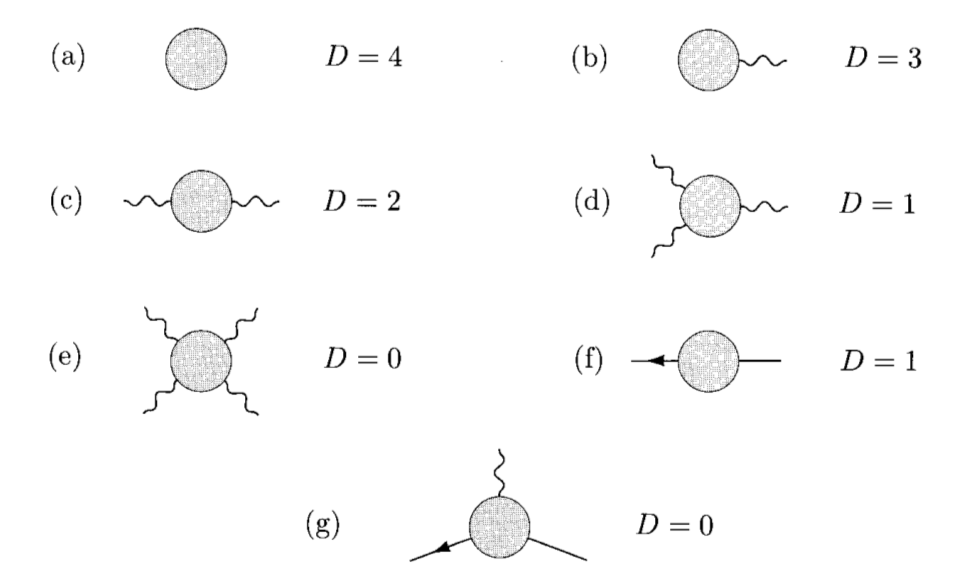
\includegraphics[width=\textwidth]{divergent_diagrams_QED.png}
\caption{The seven QED amplitudes whose superficial degree of divergence (D) is $\geq 0$.}
\label{fig:divergent_diagrams_QED}
\end{figure}


\subsection{How does renormalized perturbation theory relate the bare and physical
masses?}
In renormalized perturbation theory we begin by introducing new fields to rescale the original Lagrangian which only contains bare parameters. The next step is to introduce counterterms containing the physical parameters which splits the Lagrangian into two parts where one part now contains all infinities. The final step is to specify renormalization conditions which then fixes the physical parameters such as mass, charge or field strength. 

The common conditions to specify the physical mass is where the pole of the propagator is, in $\lambda \phi^4$-theory this simply implies that $m^2=p^2$ since the propagator is given by $\dfrac{i}{p^2-m^2+i\epsilon}$. This will define the physical mass $m$ as a function of the bare mass $m_0$ and the mass-counterterm $\delta_m$.

\pagebreak

\section{Renormalization and spontaneous symmetry
breaking}

\subsection{What is spontaneous symmetry breaking? Give a concrete example of a spontaneously broken theory.}
Subcutaneous symmetry breaking occurs when the potential term in the Lagrangian has a minima which is asymmetric with respect to the Lagrangian. Since the ground state is not at zero one needs to re-parametrize the Lagrangian around the minima in order to achieve this but this brakes the symmetry of the Lagrangian.

Consider the linear sigma model which has N symmetries with Lagrangian

\begin{equation}
L=\dfrac{1}{2}\parentheses{\partial_{\mu}\phi^i}^2 + \mu^2 \parentheses{\phi^i}^2  - \dfrac{\lambda}{4}\left[ \parentheses{\phi^i}^2 \right]
\end{equation}

where the potential term is

\begin{equation}
V \parentheses{\phi^i}=- \mu^2 \parentheses{\phi^i}^2 + \dfrac{\lambda}{4}\left[ \parentheses{\phi^i}^2 \right]
\end{equation}

which has it's minimas at $\parentheses{\phi^i_0}^2=\dfrac{\mu^2}{\lambda}$. Re-parametrizing the Lagrangian around one of this minimas breaks the $N$ symmetries and thus the symmettries are spontaneously broken.

\subsection{What is Goldstone's theorem and its implications?}
Goldstone's theorem states that every spontaneously broken symmetry with $N$ symmetries give rise to $N-1$ massless particles and $1$ massive.

This implies that spontaneously broken theories can only have one massive particle, e.g. LSW-theory where the only massive particle is the Higgs boson. The $Z$- and $W^\pm$-bosons are massless but are given mass by the Higgs mechanism.

\subsection{What are the reasons that spontaneously broken theories are renormalizable? (Assuming that the un-broken theory is.)}
Assuming that the unbroken theory is renormalizable the broken theory will also remain renormalizable since the structure of the divergent parts of the Feynman diagrams are unaffected [p.360]. The reparametrization of the Lagrangian will yield several more new divergent diagrams but they all have the same structure and thus all infinities can be absorbed into the same counterterm which renders the broken theory renormalizable as well.

\subsection{What are the basics of Wilson's approach to renormalization?}
The method of Wilson's approach to renormalization follows the following steps:

\begin{itemize}
  \item Introduce high momenta cut-off $\Lambda$
  \item Separate fields into $\hat{\phi}(k)$ where $b\Lambda < |k| < \Lambda$, $0$ otherwise and $\phi(k)$ where $|k|<b\Lambda$, $0$ otherwise and $0<b<1$.
  \item Integrate out  $\hat{\phi}(k)$ to obtain an effective Lagrangian $L_{eff}$
  \item Rescale $L_{eff}$ to obtain recursion relations for the coefficients.
\end{itemize}



\subsection{What is the Callan-Symanzik equation and how does it relate to the running of physical quantities?}


HELLO WORLD!!§
\subsection{Describe how you would chose suitable renormalization conditions.}

\end{document}